\documentclass[aspectratio=169,11pt]{beamer}
\usepackage[utf8]{inputenc}
\DeclareUnicodeCharacter{21D2}{$\Rightarrow$}
\DeclareUnicodeCharacter{21A6}{$\mapsto$}
\DeclareUnicodeCharacter{2080}{$_0$}
\DeclareUnicodeCharacter{03B3}{$\gamma$}
\DeclareUnicodeCharacter{03BA}{$\kappa$}
\DeclareUnicodeCharacter{03C3}{$\sigma$}
\DeclareUnicodeCharacter{03C9}{$\omega$}
\DeclareUnicodeCharacter{03BC}{$\mu$}
\DeclareUnicodeCharacter{03C1}{$\rho$}
\DeclareUnicodeCharacter{03B9}{$\iota$}
\DeclareUnicodeCharacter{2264}{$\leq$}
\DeclareUnicodeCharacter{2265}{$\geq$}
\DeclareUnicodeCharacter{2260}{$\neq$}
\DeclareUnicodeCharacter{2205}{$\emptyset$}
\DeclareUnicodeCharacter{2192}{$\to$}
\DeclareUnicodeCharacter{211D}{$\mathbb{R}$}
\DeclareUnicodeCharacter{2115}{$\mathbb{N}$}
\usepackage[T1]{fontenc}
\usepackage[english]{babel}
\usepackage{amsmath,amssymb}
\usepackage{booktabs}
\usepackage{graphicx}
\usepackage{tikz}
\usepackage{listings}
\usetheme{default}
\usecolortheme{seahorse}
\setbeamertemplate{navigation symbols}{}
\setbeamertemplate{footline}[frame number]
\setbeamerfont{frametitle}{size=\large}

% Lean 4 listings with pdflatex: map the Unicode characters used in the excerpts.
\lstdefinelanguage{Lean}{
  morekeywords={theorem,lemma,def,noncomputable,by,intro,apply,exact,have,rw,simp,only,
    linarith,nlinarith,omega,show,fun,let,if,then,else,Prop,Type,Finset,Monotone,Antitone},
  sensitive=true,
  morecomment=[l]{--},
  morecomment=[s]{/-}{-/},
}
\lstset{
  language=Lean,
  basicstyle=\ttfamily\scriptsize,
  keywordstyle=\color{blue!70!black}\bfseries,
  commentstyle=\color{gray},
  columns=fullflexible,
  keepspaces=true,
  breaklines=true,
  extendedchars=true,
  inputencoding=utf8,
  literate=
    {∀}{{$\forall$}}1 {ι}{{$\iota$}}1 {ℝ}{{$\mathbb{R}$}}1 {ℕ}{{$\mathbb{N}$}}1
    {→}{{$\to$}}1 {↔}{{$\leftrightarrow$}}1 {∑}{{$\sum$}}1 {∈}{{$\in$}}1
    {≤}{{$\leq$}}1 {≥}{{$\geq$}}1 {≠}{{$\neq$}}1 {⟨}{{$\langle$}}1 {⟩}{{$\rangle$}}1
    {₀}{{$_0$}}1 {Δ}{{$\Delta$}}1 {ω}{{$\omega$}}1 {σ}{{$\sigma$}}1 {ρ}{{$\rho$}}1
    {γ}{{$\gamma$}}1 {κ}{{$\kappa$}}1 {μ}{{$\mu$}}1 {¬}{{$\neg$}}1 {∧}{{$\wedge$}}1
    {·}{{$\cdot$}}1 {Ω}{{$\Omega$}}1 {⇒}{{$\Rightarrow$}}1 {↦}{{$\mapsto$}}1
    {∅}{{$\emptyset$}}1
}

\newcommand{\ind}{\mathbf 1}

\title{Quispe \& Xu (2026)}
\subtitle{\emph{Agentic Delegation and the Language Frontier of Software Developers} --- the model, and what Lean says about it}
\author{Manuel Arriola}
\date{Repository 3 \textperiodcentered{} Week of August 31 -- September 5, 2026}

\begin{document}

%================= PORTADA =============================================
\begin{frame}[plain]
  \titlepage
  \begin{center}\small
    \texttt{github.com/Arriola123456/ai-03-quispe}
  \end{center}
\end{frame}

%================= 0. LA CITA ==========================================
\begin{frame}{0 \textperiodcentered{} Start with the citation itself}
  \textbf{Asked an LLM to summarise} ``Quispe (2026), \emph{Coding Beyond Your Training:
  Claude Code and the Technological Frontier of Software Developers}.''
  Then opened the arXiv record.

  \medskip
  \footnotesize
  \begin{tabular}{@{}p{1.5cm}p{5.3cm}p{6.2cm}@{}}
    \toprule
     & Citation as given & arXiv:2605.25438 \\
    \midrule
    Title & \emph{Coding Beyond Your Training: Claude Code and the Technological Frontier of Software Developers} &
      \emph{Agentic Delegation and the \textbf{Language} Frontier of Software Developers: A Model and Evidence from Claude Code on GitHub} \\
    Authors & Quispe & Quispe \& \textbf{Xu} \\
    Date & ``2026'' & v1 2026-05-25; \textbf{v2 2026-07-07} (the Lean task pins v2) \\
    Sample & --- & 5{,}346 developers; 57 million changed files; 28-month panel \\
    \bottomrule
  \end{tabular}
  \normalsize

  \medskip
  \textbf{The discrepancy that matters:} ``technological'' vs.\ ``language'' frontier.
  Remark 1 of the paper insists the frontier is a \emph{production} frontier, not a
  \emph{skill} frontier --- the wrong title erases the paper's own caveat.
\end{frame}

%================= 1. EL PAPER Y EL PROBLEMA =========================
\begin{frame}{1 \textperiodcentered{} The paper and the agent's problem}
  \textbf{Question.} Why does a Python-only developer ship Rust the month she adopts an
  \emph{agent}, when two years of ChatGPT/Copilot did nothing of the kind?

  \medskip
  \textbf{Primitives at a fixed $(i,k,t)$.} Opportunity $\omega$, activation cost $b$,
  language skill $s\in[0,1]$, beliefs $\theta\sim N(\mu,1/\pi)$, general ability $a$,
  CARA utility $u(y)=-e^{-\rho y}$ so that $\mathrm{CE}=m-\rho\sigma^2/2$.

  \medskip
  \textbf{Three production modes} (certainty-equivalent surpluses):
  \begin{align*}
    V^S &= \omega + s\mu - \tfrac{\rho s^2}{2\pi} - b, \qquad
    V^C = V^S + \gamma s - r^C,\\
    V^D &= \omega + (1-\lambda)s\mu + \lambda a z(A) - \kappa(a,s) - r^D - b
          - \tfrac{\rho}{2}\Big[\tfrac{(1-\lambda)^2 s^2}{\pi} + \sigma_D^2(a,s,A)\Big].
  \end{align*}
  Menus $M_1=\{S,C\}$ (before) and $M_2=\{S,C,D\}$ (after); $V^g=\max_{m\in M_g}V^m$;
  language active iff $Z^g=\ind[V^g\ge 0]$; $N^g_{it}=\sum_k Z^g_{ik,t}$.

  \medskip
  \textbf{Assumption 1.} Unfamiliar: $\gamma s - r^C\le 0$; familiar: $\gamma\bar s - r^C>0$.\quad
  \textbf{Assumption 2.} $\kappa_a<0,\ \kappa_s\le 0,\ \partial\sigma_D^2/\partial a,\partial s,\partial A\le 0$.
\end{frame}

%================= 2. UMBRALES Y BANDA ================================
\begin{frame}{2 \textperiodcentered{} Thresholds and the activation band}
  Every surplus is affine in $\omega$ with slope one, so $V^m=\omega-T^m$:
  {\small
  \[
    T^S = b - s\mu + \tfrac{\rho s^2}{2\pi},\qquad
    T^C = T^S - (\gamma s - r^C),\qquad
    T^1=\min\{T^S,T^C\} = T^S-\max\{0,\gamma s - r^C\}.
  \]}
  {\small
  \[
    T^D = b-(1-\lambda)s\mu-\lambda a z(A)+\kappa(a,s)+r^D
          +\tfrac{\rho}{2}\Big[\tfrac{(1-\lambda)^2s^2}{\pi}+\sigma_D^2\Big],\qquad
    T^2=\min\{T^1,T^D\}\le T^1.
  \]}
  For an unfamiliar language Assumption 1 gives $T^1=T^S$, and the \textbf{agentic
  threshold reduction} is
  \[
    B \equiv T^1-T^D
      = \lambda\big[a z(A)-s\mu\big]-\kappa(a,s)-r^D
        +\tfrac{\rho}{2}\Big[\tfrac{(2\lambda-\lambda^2)s^2}{\pi}-\sigma_D^2(a,s,A)\Big].
  \]
  \begin{center}
  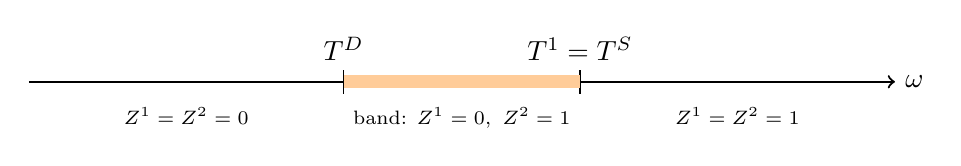
\begin{tikzpicture}[x=1cm]
    \draw[->,thick] (0,0) -- (11,0) node[right] {$\omega$};
    \draw (4,-.15) -- (4,.15) node[above] {$T^D$};
    \draw (7,-.15) -- (7,.15) node[above] {$T^1=T^S$};
    \fill[orange!40] (4,-.08) rectangle (7,.08);
    \node[below,font=\scriptsize] at (2,-.2) {$Z^1=Z^2=0$};
    \node[below,font=\scriptsize] at (5.5,-.2) {band: $Z^1=0,\ Z^2=1$};
    \node[below,font=\scriptsize] at (9,-.2) {$Z^1=Z^2=1$};
  \end{tikzpicture}
  \end{center}
\end{frame}

%================= 3. RESULTADO PRINCIPAL =============================
\begin{frame}{3 \textperiodcentered{} The main result, with all its conditions}
  \textbf{Proposition 2 (Activation band).} \emph{Consider an unfamiliar language satisfying
  Assumption 1. If $B_{ik,t}>0$, then}
  \[
    Z^2_{ik,t}-Z^1_{ik,t} \;=\; \ind\big[\,T^D_{ik,t}\le \omega_{ik,t} < T^S_{ik,t}\,\big].
  \]
  \begin{itemize}\footnotesize
    \item[(i)] \textbf{Unfamiliar language}, so Assumption 1 applies: $\gamma s - r^C\le 0\Rightarrow T^1=T^S$.
    \item[(ii)] $B>0$, i.e.\ $T^D<T^S$: the band is nonempty.
    \item[(iii)] CARA--Normal certainty equivalents behind $V^S,V^C,V^D$ (Appendix A.1);
      $\rho>0$, $\pi>0$, $\lambda\in(0,1]$.
    \item[(iv)] Menu choice is $\max$ over modes; $Z^g$ is the indicator of nonnegative surplus.
    \item[(v)] With a continuous conditional CDF $F$: $\Pr(\text{band})=F(T^S)-F(T^D)$ and
      $E[N^2-N^1]=\sum_k[F(T^1_k)-F(T^2_k)]\ge 0$ (Eq.\ 9).
  \end{itemize}
  \smallskip
  \textbf{What it does not claim} (Remark 1): $s_{ik,t}$ does not rise at adoption; the developer
  ships Rust by \emph{directing} an agent. Proposition 1 ($Z^2\ge Z^1$) is ``nearly mechanical'' --- a
  larger menu.

  \smallskip
  \textbf{What Lean added:} the identity holds \emph{without} $B>0$ (empty band, both sides $0$);
  the premise only buys nonemptiness.
\end{frame}

%================= 4. DINAMICA Y ENDPOINT =============================
\begin{frame}{4 \textperiodcentered{} Proposition 3 and the endpoint of its domain}
  Per-period first-use hazard $p^g_{ik}$; cumulative effect at horizon $s$:
  \[
    \Delta C_i(s)=\sum_{k\in U_i}\Big[(1-p^1_{ik})^{s+1}-(1-p^2_{ik})^{s+1}\Big]\ \ge 0
    \quad\text{if } p^2_{ik}\ge p^1_{ik},
  \]
  ``which in the closed-frontier benchmark $p^1_{ik}=0<p^2_{ik}$ is \textbf{strictly increasing and
  concave}.'' Appendix A.6: first difference $p^2(1-p^2)^{s+1}>0$, second $-(p^2)^2(1-p^2)^{s+1}<0$.

  \begin{columns}
    \column{0.55\textwidth}
      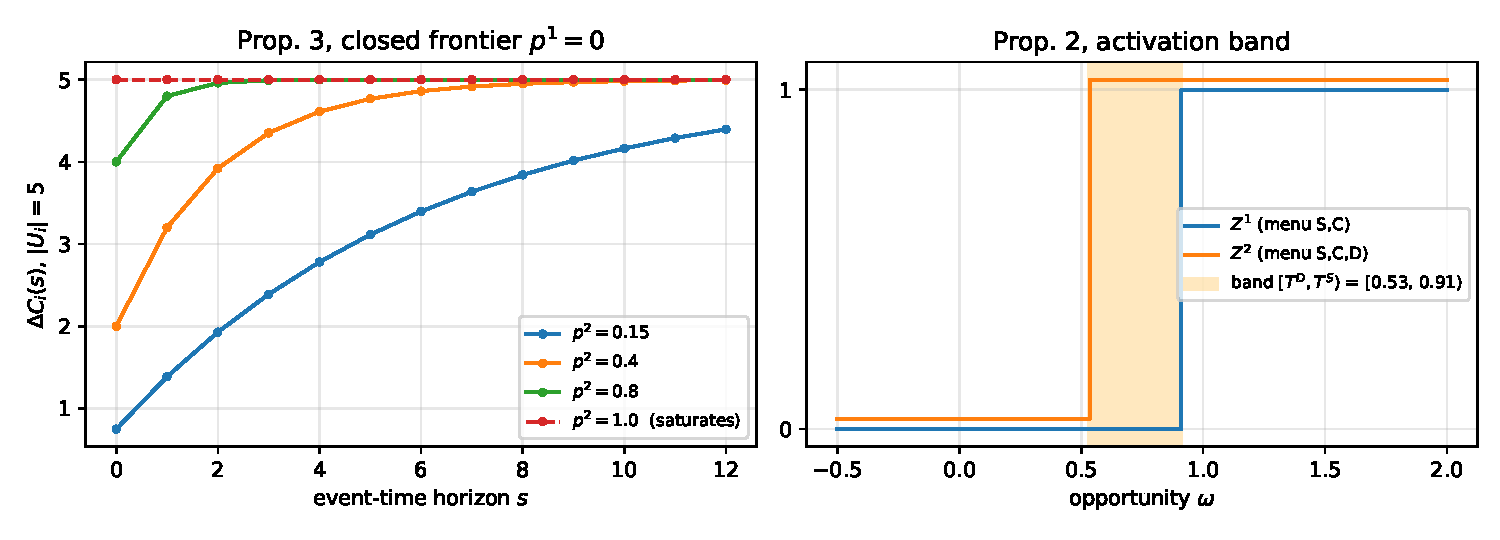
\includegraphics[width=\linewidth]{analysis/figures/prop2_prop3.pdf}
    \column{0.45\textwidth}\small
      \textbf{At $p^2=1$}, which the printed domain allows:
      $\Delta C_i(s)=|U_i|$ for every $s$ --- constant, not strictly increasing; both displayed
      inequalities are equalities.

      \medskip
      \textbf{Corrected reading:} strict increase and strict concavity for $0<p^2<1$;
      weak monotonicity on the whole domain. Lean states the strict rows with $p^2<1$ and
      proves the $p^2=1$ saturation separately.
  \end{columns}
\end{frame}

%================= 5. DOS PAPERS ======================================
\begin{frame}{5 \textperiodcentered{} Two papers, one phenomenon, one modelling choice}
  \begin{columns}[T]
    \column{0.48\textwidth}
      \textbf{Aouad--Lykouris--Zhong (week 1)}\\[2pt]
      AI is a \emph{perfectly substitutable input} on the \emph{intensive} margin of a task the
      worker already does:
      \[ x=s+e+a,\qquad \max_{e\ge 0} p(s+e+a)-\gamma e .\]
      Assistance crowds out effort; effort builds skill $\Rightarrow$ \textbf{deskilling}.
    \column{0.48\textwidth}
      \textbf{Quispe--Xu}\\[2pt]
      Agentic AI is a \emph{new production mode} on the \emph{extensive} margin, with its own
      threshold that does not load on $s$:
      \[ V^2=\max\{V^S,V^C,V^D\}\ \ge\ V^1 .\]
      It adds options instead of replacing inputs $\Rightarrow$ \textbf{frontier expansion}.
  \end{columns}

  \medskip
  \textbf{The single choice.} Whether AI enters \emph{inside} the production function of an
  existing task (a substitute for $e$, so it displaces the thing that builds $s$) or \emph{beside}
  it as an alternative technology for a task that was infeasible. Neither paper needs the other's
  mechanism to be false; they model different margins. A model with both would have deskilling in
  familiar languages and expansion in unfamiliar ones --- which is, roughly, the paper's own
  Figure 1 read together with Remark 1.
\end{frame}

%================= 6. ANALITICO =======================================
\begin{frame}{6 \textperiodcentered{} What I did analytically}
  \begin{columns}[T]
    \column{0.42\textwidth}
      \includegraphics[page=2,height=0.72\textheight]{hand/derivacion-a-mano.pdf}
    \column{0.56\textwidth}\small
      \textbf{By hand (\texttt{hand/}, 5 pages).} The step I did not want to take on trust:
      the CARA--Normal certainty equivalent. With $Y\sim N(m,\sigma^2)$ and $u=-e^{-\rho y}$,
      the MGF gives $E[-e^{-\rho Y}]=-\exp(-\rho m+\rho^2\sigma^2/2)$, hence
      $\mathrm{CE}=m-\rho\sigma^2/2$. Then $V^S$ from $Y^S=\omega+s\theta-b$
      ($\mathrm{Var}=s^2/\pi$), $V^C$, and $V^D$ with
      $\mathrm{Var}[Y^D]=(1-\lambda)^2s^2/\pi+\sigma_D^2$.

      \medskip
      \textbf{Threshold algebra.} $T^S-T^D$ reduces to Equation (7) because
      $\tfrac{\rho}{2}\tfrac{s^2}{\pi}\big[1-(1-\lambda)^2\big]=\tfrac{\rho}{2}(2\lambda-\lambda^2)\tfrac{s^2}{\pi}$.

      \medskip
      \textbf{Endpoint checks.} $\lambda=1$: fine (human match risk vanishes).
      $\pi\to\infty$: fine. $B\le 0$: identity (8) still holds, band empty.
      $p^2=1$: Proposition 3's strict claims fail. Comparative static ``$B$ larger for
      higher $a$'' needs $z(A)\ge 0$ and $\rho\ge 0$, which the text leaves implicit.
  \end{columns}
\end{frame}

%================= 7. COMPUTACIONAL ===================================
\begin{frame}{7 \textperiodcentered{} What I did computationally --- and with which tools}
  \footnotesize
  \textbf{EconCSLib workflow} (\texttt{nikhgarg/EconCSLib}, commit \texttt{cf500b74}, Lean/Mathlib \texttt{v4.30.0-rc2}, WSL2 Ubuntu 26.04):
  \begin{enumerate}
    \item pin the v2 PDF outside the repo (SHA-256 \texttt{cddc0487\ldots3d35}); \texttt{init-spec};
    \item fill the \textbf{statement spec}: 15 targets, each with source locator, literal source
      statement and a transparent Lean proposition;
    \item \texttt{paper\_contribution.py new} $\to$ scaffold (Lean-validates every Spec);
    \item \texttt{MainTheorems.lean} (model, threshold algebra) + \texttt{ProofInterface.lean} (15 endpoints);
    \item \texttt{lake build QX26AgenticDelegation}: \textbf{Build completed successfully (4000 jobs)};
      \texttt{check --fast}: \textbf{exit 0}; full \texttt{check}: build and status lanes pass, stops at the
      conclusion-provenance audit (needs the LLM-as-judge sidecars; \texttt{lean/docs/CHECK\_FULL\_OUTPUT.txt}).
  \end{enumerate}
  \textbf{Result.} 15/15 Specs proved, no \texttt{sorry}; status \emph{partially formalized}
  (two Proposition 3 rows carry the added $p^2<1$; semantic audits pending).

  \smallskip
  \textbf{Who ran what --- the blocker.} Codex \texttt{gpt-5.6-sol}/\texttt{xhigh} was launched exactly as
  required; it read the skills, wrote the placeholder spec, tested a scratch file (parse errors:
  \texttt{⇒} for \texttt{↦}) and died: \texttt{usage\_limit\_exceeded}, \emph{``Your workspace is out of
  credits.''} Steps 2--5 were done with Claude Code --- disclosed in \texttt{prompts.md} and
  \texttt{lean/docs/RUN\_LOG.md}; nothing in \texttt{lean/} is presented as the Codex run.
\end{frame}

%================= 8. SLIDE LEAN OBLIGATORIA (I) =======================
\begin{frame}[fragile]{8 \textperiodcentered{} Lean: Proposition 3 --- from the equation to a checked proof}
  \small\textbf{Paper claim (Prop.\ 3, A.6).} For $p^1=0<p^2$,\;
  $\Delta C(s)=\sum_{k\in U}\big[(1-0)^{s+1}-(1-p^2_k)^{s+1}\big]$ is strictly increasing in $s$.

  \smallskip
  \textbf{Lean statement} (\texttt{PaperInterface.lean}, transparent Spec):
\begin{lstlisting}
def paper_proposition_3_closed_frontier_strictly_increasingSpec : Prop :=
  ∀ {ι : Type} (U : Finset ι) (p2 : ι → ℝ) (s : ℕ),
    U.Nonempty → (∀ k, 0 < p2 k) → (∀ k, p2 k < 1) →
      ∑ k ∈ U, ((1 - (0 : ℝ)) ^ (s + 1) - (1 - p2 k) ^ (s + 1))
        < ∑ k ∈ U, ((1 - (0 : ℝ)) ^ (s + 2) - (1 - p2 k) ^ (s + 2))
\end{lstlisting}
  \textbf{Proof fragment} (\texttt{ProofInterface.lean}):
\begin{lstlisting}
  apply Finset.sum_lt_sum_of_nonempty hU          -- needs U ≠ ∅
  intro k _
  have hq0 : 0 < 1 - p2 k := by linarith [h1 k]   -- needs p2 k < 1 (added)
  have hq1 : 1 - p2 k < 1 := by linarith [h0 k]   -- needs 0 < p2 k
  have := pow_lt_pow_right_of_lt_one₀ hq0 hq1 (show s + 1 < s + 2 by omega)
  simp only [sub_zero, one_pow]; linarith
\end{lstlisting}
  \textbf{Reading.} $U_i\mapsto$ \texttt{Finset}, hazards $\mapsto$ \texttt{p2 : ι → ℝ}, horizon $\mapsto$
  \texttt{s : ℕ}; the strict step \texttt{pow\_lt\_pow\_right\_of\_lt\_one₀} needs $0<1-p<1$.
\end{frame}

%================= 9. SLIDE LEAN OBLIGATORIA (II) ======================
\begin{frame}[fragile]{9 \textperiodcentered{} Lean: Proposition 3 --- the endpoint, and what Lean actually verifies}
  \small\textbf{The endpoint theorem} (\texttt{MainTheorems.lean}):
\begin{lstlisting}
theorem cumulative_effect_saturates_at_hazard_one {ι : Type} (U : Finset ι)
    (p2 : ι → ℝ) (s : ℕ) (h : ∀ k, p2 k = 1) :
    ∑ k ∈ U, ((1 - (0 : ℝ)) ^ (s + 1) - (1 - p2 k) ^ (s + 1))
      = ∑ k ∈ U, ((1 - (0 : ℝ)) ^ (s + 2) - (1 - p2 k) ^ (s + 2)) := by
  apply Finset.sum_congr rfl; intro k _; rw [h k]; simp
\end{lstlisting}
  \begin{itemize}\small
    \item \textbf{Objects.} $U_i\mapsto$ \texttt{U : Finset ι}; $p^2_{ik}\mapsto$ \texttt{p2 k}; the horizon
      $s\in\mathbb N$; $\Delta C_i(s)$ is written out as the source sum with $p^1=0$ kept explicit as
      \texttt{(1 - (0 : ℝ))}.
    \item \textbf{Assumptions.} The source says only $p^1=0<p^2$. Lean would not close the strict
      inequality with that: \texttt{pow\_lt\_pow\_right\_of\_lt\_one₀} demands $1-p^2<1$ \emph{and}
      $0<1-p^2$, i.e.\ $0<p^2<1$; the sum lemma demands $U\neq\emptyset$.
    \item \textbf{Conclusion.} Lean verifies the source claim \textbf{only after adding} $p^2<1$ and
      $U\neq\emptyset$; the second theorem proves that at $p^2=1$ the two sides are \emph{equal}, so
      the printed strict claim is false on its stated domain.
    \item \textbf{Check.} \texttt{lake build QX26AgenticDelegation}: Build completed successfully (4000 jobs);
      \texttt{paper\_contribution.py check --fast}: exit 0; no \texttt{sorry}.
  \end{itemize}
\end{frame}

%================= 10. LEAN: PROP 2, ENUNCIADO =========================
\begin{frame}[fragile]{10 \textperiodcentered{} Lean: Proposition 2 --- the statement, exactly as printed}
  \small\textbf{Paper claim.} Assumption 1 and $B>0$ $\Rightarrow$ $Z^2-Z^1=\ind[T^D\le\omega<T^S]$.
  \quad(\texttt{lam} $=\lambda$, \texttt{prec} $=\pi$, \texttt{z} $=z(A)$, \texttt{κ}, \texttt{σ} at fixed $(i,k,t)$)
\begin{lstlisting}
def paper_proposition_2_activation_bandSpec : Prop :=
  ∀ ω s μ prec b ρ γ rC lam a z κ rD σ : ℝ,
    let VS := ω + s * μ - ρ * s ^ 2 / (2 * prec) - b
    let VC := VS + γ * s - rC
    let VD := ω + (1 - lam) * s * μ + lam * a * z - κ - rD - b
                - ρ / 2 * ((1 - lam) ^ 2 * s ^ 2 / prec + σ)
    let TS := b - s * μ + ρ * s ^ 2 / (2 * prec)
    let TD := b - (1 - lam) * s * μ - lam * a * z + κ + rD
                + ρ / 2 * ((1 - lam) ^ 2 * s ^ 2 / prec + σ)
    γ * s - rC ≤ 0 → 0 < TS - TD →
      (if 0 ≤ max (max VS VC) VD then (1 : ℝ) else 0)
          - (if 0 ≤ max VS VC then (1 : ℝ) else 0)
        = if TD ≤ ω ∧ ω < TS then (1 : ℝ) else 0
\end{lstlisting}
  \textbf{Reading.} Equations (1)--(3) are the \texttt{let}s; the menus are the nested \texttt{max};
  $Z^g$ is the \texttt{if}; Assumption 1 is \texttt{γ * s - rC ≤ 0}; $B>0$ is \texttt{0 < TS - TD}.
  Every quantifier and inequality of the source is visible --- nothing hides behind a definition.
\end{frame}

%================= 11. LEAN: PROP 2, PRUEBA ============================
\begin{frame}[fragile]{11 \textperiodcentered{} Lean: Proposition 2 --- the proof route}
  \small\textbf{Route.} $V^C\le V^S$ (Assumption 1) $\Rightarrow$ \texttt{max VS VC = VS}; rewrite
  $V^S=\omega-T^S$, $V^D=\omega-T^D$ (\texttt{ring}); then one real lemma:
\begin{lstlisting}
theorem band_indicator {ω TS TD : ℝ} (hlt : TD < TS) :
    (if 0 ≤ max (ω - TS) (ω - TD) then (1:ℝ) else 0) - (if 0 ≤ ω - TS then (1:ℝ) else 0)
      = if TD ≤ ω ∧ ω < TS then (1:ℝ) else 0 := by
  have hmax : max (ω - TS) (ω - TD) = ω - TD := max_eq_right (by linarith)
  rw [hmax]
  by_cases hS : TS ≤ ω        -- case 1: ω ≥ TS  → 1 - 1 = 0, band indicator 0
  · ...                       -- case 2: TD ≤ ω < TS → 1 - 0 = 1, band indicator 1
  · by_cases hD : TD ≤ ω      -- case 3: ω < TD  → 0 - 0 = 0
    ...
\end{lstlisting}
  \begin{itemize}\small
    \item Each case is closed by \texttt{if\_pos}/\texttt{if\_neg} on the three conditions and
      \texttt{norm\_num} on the resulting $1-1$, $1-0$, $0-0$.
    \item Lean verifies the source claim \textbf{exactly}: no added hypothesis, no changed domain.
    \item \textbf{Extension} \texttt{activation\_band\_general} drops \texttt{0 < TS - TD}: when
      $T^D\ge T^S$ the band is empty and both sides are $0$ --- the premise $B>0$ only makes the
      band nonempty.
  \end{itemize}
\end{frame}

%================= 12. LA IA =========================================
\begin{frame}{12 \textperiodcentered{} Where I did not believe the AI}
  \begin{columns}[T]
    \column{0.36\textwidth}
      \includegraphics[page=5,height=0.70\textheight]{hand/derivacion-a-mano.pdf}
    \column{0.62\textwidth}\footnotesize
      \textbf{Claim 1 (an LLM, cold).} A confident summary of ``\emph{Coding Beyond Your Training}''
      --- a title that does not exist, one author instead of two.
      \textbf{Verdict: fabricated}; the arXiv record settles it (slide 0).

      \medskip
      \textbf{Claim 2 (the risk term in $V^D$).} Delegation shrinks the human-match variance from
      $s^2/\pi$ to $(1-\lambda)^2s^2/\pi$ and adds $\sigma_D^2$; the penalty is $\tfrac{\rho}{2}$ times
      the variance. I did not take the CE formula or the $(1-\lambda)^2$ on trust: MGF $\to$
      $\mathrm{CE}=m-\rho\sigma^2/2$ $\to$ $\mathrm{Var}[(1-\lambda)s\theta]=(1-\lambda)^2s^2/\pi$
      (on screen). \textbf{Verdict: Equation (3) is right as printed.}

      \medskip
      \textbf{Claim 3 (Codex's draft Lean).} Wrote \texttt{⇒} where Lean 4 wants \texttt{↦}/\texttt{=>};
      never reached a statement. \textbf{Verdict: syntax, not mathematics} --- but it is why every Spec
      was tested in a scratch file before scaffolding.

      \medskip
      \textbf{Claim 4 (the paper itself).} ``Strictly increasing and concave'' for $p^1=0<p^2$.
      \textbf{Verdict: false at $p^2=1$}; Lean proves the saturation (slide 9).
  \end{columns}
\end{frame}

%================= 13. LA TRAMPA ======================================
\begin{frame}{13 \textperiodcentered{} This week's trap: where the argument is weakest}
  \begin{itemize}\footnotesize
    \item \textbf{Does the mechanism need an \emph{agent}?} In the model, no. What creates the band is
      that mode $D$'s value \emph{does not load on $s$} while mode $C$'s value is $\gamma s$
      (Assumption 1). Any assistance worth $\gamma'-r$ with $\gamma'$ independent of $s$ would lower
      $T^1$ for unfamiliar languages just as well. ``Agent'' is a \emph{restriction on the shape of the
      assistance technology}, not a derived necessity. The paper's defence is Section 3 --- the
      generational boundary is datable, so the shape assumption is testable --- an empirical argument,
      not a theorem.
    \item \textbf{Endpoints.} $p^2=1$ breaks Proposition 3's strict claims (proved). $B>0$ is not
      needed for Proposition 2's identity (proved). The comparative static after (7) needs
      $z(A)\ge 0$, $\rho\ge 0$ (added in Lean). Nothing breaks at $\lambda=1$.
    \item \textbf{Representation gaps Lean makes visible.} Propositions 4 and 5 are stated over
      abstract hazards $p_i(a_i,A)$ and entry costs $c_r(\ell,g)$; the link from $Z^2-Z^1$ to those
      objects is assumed, exactly as in the source proofs. Verification certifies the \emph{algebra},
      not the \emph{economics} of the reduced form.
    \item \textbf{Selection into adoption} (empirical; flagged by the authors): the event-time estimates
      are associations. The model cannot distinguish a lower $T^D$ from a project shock that raises
      $\omega$ at adoption --- both put $\omega$ in the band.
  \end{itemize}
\end{frame}

%================= 14. CIERRE =========================================
\begin{frame}{14 \textperiodcentered{} What is in the repository}
  \texttt{github.com/Arriola123456/ai-03-quispe}
  \begin{itemize}
    \item \texttt{README.md} --- question, agent's problem, Proposition 2 with all its conditions, the Aouad contrast.
    \item \texttt{prompts.md} --- raw: the Codex session (107 tool calls, then \texttt{usage\_limit\_exceeded})
      and the Claude Code session, including every Lean error hit and fixed.
    \item \texttt{hand/derivacion-a-mano.pdf} --- CE via the MGF; $V^S$, $V^C$, $V^D$.
    \item \texttt{lean/} --- the EconCSLib folder as generated: 15 Specs, 15 closed proofs, validation report,
      dependency DAG, audit stubs, \texttt{docs/RUN\_LOG.md}, \texttt{docs/CHECK\_FULL\_OUTPUT.txt}.
    \item \texttt{analysis/} --- the numerical check behind slide 4.
  \end{itemize}
  \medskip
  \textbf{One sentence.} The model is right about the band and wrong about one endpoint;
  Lean found the endpoint because it would not let ``$0<p^2$'' stand in for ``$0<p^2<1$''.
\end{frame}

\end{document}
